\documentclass[10pt,a4paper]{article}

\usepackage[latin1]{inputenc}
\usepackage{amsmath}
\usepackage{amsfonts}
\usepackage{amssymb}
\usepackage{graphicx}
\usepackage{listings}
\title{Assignment No :A1}
\date{}
\author{Roll No.4431}


\begin{document}
\maketitle
\section{Title:}
Binary Search Tree

\section{Problem Definition}
Using Divide and Conquer Strategies design a cluster/Grid of BBB or Rasberi pi or Computers in network
to run a function for Binary Search Tree using C /C++/ Java/Python/ Scala. 

\section{Learning Objectives}
\begin{enumerate}
\item To understand the concept of a binary search tree.
\item To understand applications of a distributed architecture.
\item To form clusters using BBB.
\end{enumerate}

\section{Learning Outcomes}
\begin{enumerate}
\item Ability to analyze problems as data structures.
\item Understanding of grid computing.
\item Basic understanding about what trees are AND how they are represented.
\end{enumerate}


\section{Related Mathematics}
Let S be the solution perspective of the given problem.
\\\\The set S is defined as:
\\\\$S=\lbrace\ s,e,X,Y,F,DD,NDD,S_{c},F_{c}|\varnothing_{s}\rbrace$
\\\\Where,
\\\\s= Start state,  Such that $Y=\lbrace \varnothing \rbrace$ 
\\\\e= End state 
\\\\X= Input Set.
\\\\$X=\lbrace$ seq(x) $\mid$ x $\in$ Natural numbers $\rbrace$
\\\\Y=Output set.
\\\\$Y=\lbrace Binary Search Tree \rbrace $
\\\\F= Set of functions used.
\\\\F=$\lbrace mkTree(),insert(), delete(), print() \rbrace$
\\\\mkTree()= function to generate a binary search tree from the given numbers.
\\\\insert()= function to insert an element in the tree.
\\\\delete()= function to delete an element from the tree.
\\\\print()= function to print the tree in a specific order.
\\\\DD=Deterministic data.
\\DD=
\begin{enumerate}
\item tree follows proper constraints.
\item search element exists.
\item tree terminates.
\end{enumerate}
NDD= Non-deterministic data.
\\NDD= $\cup$ - DD


\section{State Transition diagram}
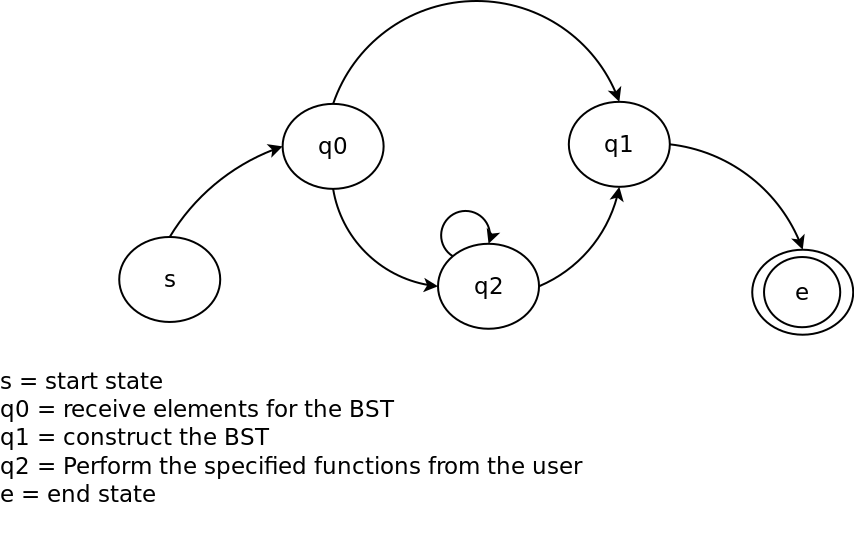
\includegraphics[scale=0.30]{stdg.png}

\section{Concepts related theory}
\subsection{Divide and Conquer : }
\begin{itemize}
		\item Given a function to compute on an inputs the divide and conquer strategy suggest splitting the input into k distinct input sets ,such that 1<k<n yielding k sub problems.
		\item These sub problems must be solve and then method must be found to combine the sub solution into a solution of a whole.
		\item If the sub problems are relatively large then the divide and conquer strategy can be possibly reapplied.
		\item Often the sub problems are of the same type as the same original problem for which the reapplication of divide and conquer principle is naturally expressed by a recursive algorithm.
\end{itemize}

\subsection{Binary Search Tree : }
	\begin{itemize}
		\item A binary search tree is a tree where each node has a left and right child. Either child, or both children, may be missing. Figure 3-2 illustrates a binary search tree. Assuming k represents the value of a given node, then a binary search tree also has the following property: all children to the left of the node have values smaller than k, and all children to the right of the node have values larger than k. The top of a tree is known as the root, and the exposed nodes at the bottom are known as leaves. In Figure 3-2, the root is node 20 and the leaves are nodes 4, 16, 37, and 43. The height of a tree is the length of the longest path from root to leaf. For this example the tree height is 2. 
	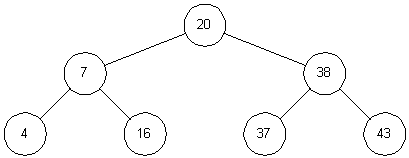
\includegraphics[scale = 0.8]{A1_01}

    	\item To search a tree for a given value, we start at the root and work down. For example, to search for 16, we first note that 16 < 20 and we traverse to the left child. The second comparison finds that 16 > 7, so we traverse to the right child. On the third comparison, we succeed. 
        \item Each comparison results in reducing the number of items to inspect by one-half. In this respect, the algorithm is similar to a binary search on an array. However, this is true only if the tree is balanced. For example, Figure 3-3 shows another tree containing the same values. While it is a binary search tree, its behavior is more like that of a linked list, with search time increasing proportional to the number of elements stored. 
   	   	
			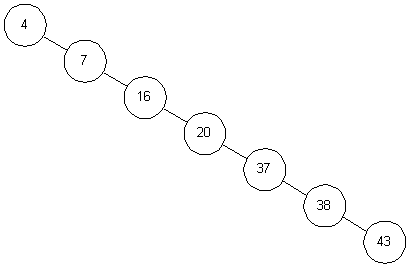
\includegraphics[scale = 0.8]{A1_02}
		
    	\subsubsection{Insertion and deletion : }
        \begin{itemize}
			\item Let us examine insertions in a binary search tree to determine the conditions that can cause an unbalanced tree. To insert an 18 in the tree in Figure 3-2, we first search for that number. This causes us to arrive at node 16 with nowhere to go. Since 18 > 16, we simply add node 18 to the right child of node 16 (Figure 3-4). 
            \item Now we can see how an unbalanced tree can occur. If the data is presented in an ascending sequence, each node will be added to the right of the previous node. This will create one long chain, or linked list. However, if data is presented for insertion in a random order, then a more balanced tree is possible. 
            \item Deletions are similar, but require that the binary search tree property be maintained. For example, if node 20 in Figure 3-4 is removed, it must be replaced by node 37. This results in the tree shown in Figure 3-5. The rationale for this choice is as follows. The successor for node 20 must be chosen such that all nodes to the right are larger. Therefore we need to select the smallest valued node to the right of node 20. To make the selection, chain once to the right (node 38), and then chain to the left until the last node is found (node 37). This is the successor for node 20. 
		\end{itemize}
	\end{itemize}
			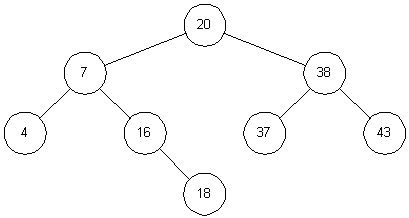
\includegraphics[scale = 0.8]{A1_03}
		
			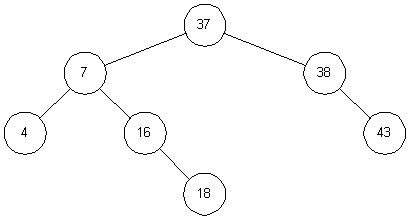
\includegraphics[scale = 0.8]{A1_04}
		

\section{Program Listing}
\begin{lstlisting}
# client.py

import socket, pickle

HOST = 'localhost'
PORT = 50007
s = socket.socket(socket.AF_INET, socket.SOCK_STREAM)
s.connect((HOST, PORT))
arr = [7,1,9,12,6,88,11,65]
data_string = pickle.dumps(arr)
s.send(data_string)
s.close()





# server.py

import socket, pickle

class BST:
    def __init__(self, val=None):
        self.left = None
        self.right = None
        self.val = val

    def __str__(self):
        return "[%s, %s, %s]" % (self.left, str(self.val), self.right)

    def isEmpty(self):
        return self.left == self.right == self.val == None

    def insert(self, val):
        if self.isEmpty():
            self.val = val
        elif val < self.val:
            if self.left is None:
                self.left = BST(val)
            else:
                self.left.insert(val)
        else:
            if self.right is None:
                self.right = BST(val)
            else:
                self.right.insert(val)

HOST = 'localhost'
PORT = 50007
s = socket.socket(socket.AF_INET, socket.SOCK_STREAM)
s.bind((HOST, PORT))
s.listen(1)
conn, addr = s.accept()
print 'Connected by', addr
while 1:
    data = conn.recv(4096)
    if not data: break
    data_arr = pickle.loads(data)
conn.close()
print 'Received', repr(data_arr)

iter = BST()
for i in data_arr:
	#print i
	iter.insert(i)
print iter

\end{lstlisting}

\newpage
\section{Output}
\begin{lstlisting}
botman@botmatrix:~$ python server.py
Connected by ('127.0.0.1', 52393)
Received [7, 1, 9, 12, 6, 88, 11, 65]
[[None, 1, [None, 6, None]], 7, [None, 9, [[None, 11, None], 12, [[None, 65, None], 88, None]]]]


botman@botmatrix:~$ python client.py

\end{lstlisting}

\section{Testing}

\vspace{20px}

\subsection{Positive Testing}
\begin{center}
	\begin{tabular}
		{|c|c|c|c|c|}\hline
		{\bf Sr. No.}		&{\bf Test Condition }	&{\bf Steps to be Executed}	&{\bf Expected Result} & Actual Result \\ \hline
		{1}	&	{Enter the Key to be found}& {Press Enter}		&  {Display} & {Same as Expected}\\ 
		\hline
		{2}	&	{Find the key at particular position}& {Press Enter}		&  {Position of key} & {Same as Expected}\\ 
		\hline
		
	\end{tabular}\\ 
\end{center}

\subsection{Negative Testing}
\begin{center}
	\begin{tabular}
		{|c|c|c|c|c|}\hline
		{\bf Sr. No.}		&{\bf Test Condition }	&{\bf Steps}	&{\bf Expected Result} & Actual Result \\ \hline
		{1}	&	{Enter the Key not in array}& {Give key}&  {If not display error message} & {Display position of key}\\
		\hline
		
	\end{tabular}\\ 
\end{center}

\section{CONCLUSION :}
Thus we have successfully studied Divide and Conquer Strategies to design a cluster/Grid of Computers in network to run a function for Binary Search Tree using Python.\\\\

\end{document}